\section{Technologies used}

\subsection{JAVA: Object Oriented Programming Language}
The use of Java as programming language guarantees an easy development, thanks to the large amount of APIs for the communication among processes and other processes or with a DBMS. Furthermore the object oriented model give us an ease in mantainment and a intrinsecal modularity of the application.
\subsection{MySQL: Relational Database Management System}
MySQL is one of the most used relational database management systems and it's open source. Furthermore it was a design constraint to use this DBMS for the development of this project.

\section {Client Side Implementation}
\subsection {User Interface}
\subsection {Request Handler}
\section {Server Side Implementation}
\subsection {Request Handler}
\subsection {DBManager}
\subsection {Database}
The following diagram is the logical representation of the DB used by the application.
The Database used in this application is composed of three tables:
\begin{enumerate}
	\item User:
\begin{tabular}{|l|l|l|}
\hline
	Attribute  & Type \\
\hline
userID            & 0     & zero          \\
username         & 1     & uno           \\
password           & 2     & due           \\
arancio        & 3     & tre           \\
giallo          & 4     & quattro       \\
verde           & 5     & cinque        \\
blu             & 6     & sei           \\
viola           & 7     & sette         \\
grigio          & 8     & otto          \\
bianco          & 9     & nove          \\
argento         & 10 \% &               \\
oro             & 5 \%  &               \\
                & 2 \%  &               \\
                & 1 \%  &               \\
\hline
\end{tabular}
\item Restaurant:
\begin{tabular}{|l|l|l|l|}
\hline
          & Numero        &       \\
\hline
nero            & 0     & zero          \\
marrone         & 1     & uno           \\
rosso           & 2     & due           \\
arancio         & 3     & tre           \\
giallo          & 4     & quattro       \\
verde           & 5     & cinque        \\
blu             & 6     & sei           \\
viola           & 7     & sette         \\
grigio          & 8     & otto          \\
bianco          & 9     & nove          \\
argento         & 10 \% &               \\
oro             & 5 \%  &               \\
                & 2 \%  &               \\
                & 1 \%  &               \\
\hline
\end{tabular}
\item Reservation:
\begin{tabular}{|l|l|l|l|}
\hline
          & Numero        &       \\
\hline
nero            & 0     & zero          \\
marrone         & 1     & uno           \\
rosso           & 2     & due           \\
arancio         & 3     & tre           \\
giallo          & 4     & quattro       \\
verde           & 5     & cinque        \\
blu             & 6     & sei           \\
viola           & 7     & sette         \\
grigio          & 8     & otto          \\
bianco          & 9     & nove          \\
argento         & 10 \% &               \\
oro             & 5 \%  &               \\
                & 2 \%  &               \\
                & 1 \%  &               \\
\hline
\end{tabular}
\end{enumerate}
\begin{figure}
  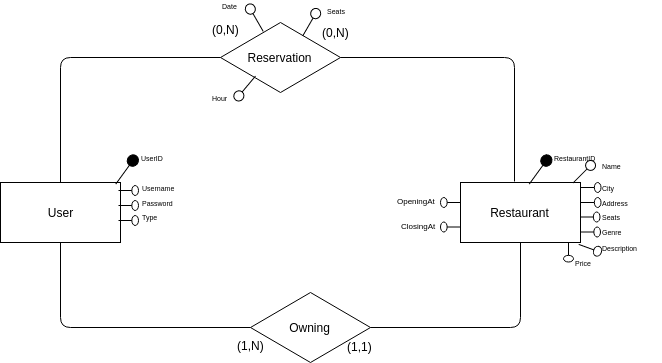
\includegraphics[width=\linewidth]{ERLSMSD.png}
  \caption{ER Diagram.}
  \label{figureER}
\end{figure}
\section {Java Beans Implemented}

\pagebreak